\chapter{Theoretische Grundlagen}

% -> Nur Theorie, die später auch verwendet wird, nichts einfach so einführen

% -> Voraussetzung: Basiswissen WI-Studium

\section{Geschäftsprozessanalyse und -optimierung}

\subsubsection{Geschäftsprozess}\label{sec:Kapitel211}

Um eine höhere Effizienz und somit auch Kosteneinsparungen  zu erzielen, haben Unternehmen immer wieder Aufgaben und Arbeitsabläufe analysiert. Bei klassischen Konzepten, wie der Aufbau- und Ablauforganisation sind hierbei meist einzelne Aufgaben oder kurze Arbeitsaufläufe im Fokus. Meistens fanden die Analyse im Rahmen von einzelnen Organisationseinheiten oder Stellen statt, wie diese ihre Aufgaben effizienter bewältigen können. Durch das Konzept des Geschäftsprozesses (im Folgenden mit ''GP'' abgekürzt) wandelt sich diese Betrachtung zu einer ganzheitlicheren Sichtweise, bei der längere Wertschöpfungsketten zur Erfüllung einer grö\ss eren Aufgabe betrachtet werden und die Grenzen einzelner Organisationsstrukturen eine untergeordnete Rolle spielen. Somit liegt der Fokus weniger auf den einzelnen Aufgaben im Sinne der Arbeitsteilung, sondern der sequenziellen Grundstruktur. \footcite[Vgl.][S. 5]{theorie_staud_geschäftsprozessanalyse_2006}

Staud definiert GP als eine zusammenhängende abgeschlossene Folge von Tätigkeiten, die zur Erfüllung einer betrieblichen Aufgabe notwendig sind. Die Tätigkeiten werden von Aufgabenträgern in organisatorischen Einheiten unter Nutzung der benötigten Produktionsfaktoren geleistet. Unterstützt wird die Abwicklung der GP durch das Informations- und Kommunikationssystem des Unternehmens. \parencite[Vgl.][S. 9]{theorie_staud_geschäftsprozessanalyse_2006} Ein GP kann auf unterschiedlichen Aggregationsebenen dargestellt werden: Beispielsweise die Abwicklung eines Auftrags vom Eingang bis zur Auslieferung, aber auch auf kleinteiligerer Ebene die Zahlungsabwicklung. Ausschlaggebend für diese Abgrenzung als eigener GP sind nach einer Studie der LMU unter deutschen Gro\ss konzernen die folgenden Kriterien: Der Prozess ist wertschöpfend, funktionsübergreifend, kundenorientiert und hat eine strategische Bedeutung. Zudem müssen ein Prozessverantwortlicher und Ziele bzw. Messgrö\ss en vorhanden sein.\footcite[Vgl.][S. 19]{theorie_koch_studie_kriterien_geschäftsprozess_2003} 

Grundsätzlich können GP drei Kategorien zugeordnet werden: Steuerungsprozesse, Kerngeschäftsprozesse und unterstützende Prozesse.

\begin{figure}[H]
    \centering
    \includegraphics[height=5cm]{Bilder/Geschäftsprozesse_Arten.png}
    \caption[Steuerungs-, Kern- und Unterstützungsprozesse]{Steuerungs-, Kern- und Unterstützungsprozesse. Darstellung nach \cite[][S. 44]{theorie_gadatsch_grundkurs_geschäftsprozessmanagement_2010}}
    \label{fig:Geschäftsprozesse_Arten}
\end{figure}

Steuerungsprozesse dienen nach Abbildung \ref{fig:Geschäftsprozesse_Arten} der Steuerung und dem Zusammenspiel aller anderen GP. Beispiele für diese Art sind strategische Planungs-, operative Führungs- oder Controlling-Prozesse. Sie Bilden den unternehmerischen Rahmen um alle Prozesse der betrieblichen Leistungserstellung und -unterstützung. Kerngeschäftsprozesse sind GP, die hauptsächlich für die Wertschöpfung verantwortlich sind. Sie decken den gesamten Leistungsprozess von der Produktentwicklung bis zur Auslieferung ab und sind wettbewerbskritisch. Unter diese Kategorie fallen \zB Entwicklung, Produktion, Vertrieb im Beispiel eines Automobilherstellers. Unterstützungsprozesse tragen nicht direkt oder nur wenig zur Leistungserstellung bei, sind aber für die Funktionsfähigkeit des Unternehmens dennoch wichtig. Finanzbuchhaltung, Personalwesen oder Compliance sind Beispiele für diesen Typ. \footcite[Vgl.][S. 44]{theorie_gadatsch_grundkurs_geschäftsprozessmanagement_2010}

GP lassen sich nach Berkau in betriebswirtschaftliche und technische GP unterteilen, wobei sich technische GP auf die primäre Leistungserstellung und betriebswirtschaftliche GP auf kaufmännische Tätigkeiten beziehen. \parencite[Vgl.][S. 27]{theorie_berkau_arten_geschäftsprozesse_1998} Beispiele für technische GP wären die Produktion eines Autos im Falle eines Automobilherstellers; für betriebswirtschaftliche GP wäre es die Bearbeitung eines Lieferantenvertrags im Einkauf. In dieser Arbeit wird das Hauptaugenmerk auf betriebswirtschaftlichen GP liegen. \footcite[Vgl.][S. 10]{theorie_staud_geschäftsprozessanalyse_2006} GP lassen sich nach zudem nach ihrer Komplexität und Wertschöpfung unterteilen, wie in Abbildung \ref{fig:Geschäftsprozess_Einordnung2} nachfolgend dargestellt wird:

\begin{figure}[H]
    \centering
    \includegraphics[height=6cm]{Bilder/Geschäftsprozess_Einordnung2.png}
    \caption[Einordnung von Geschäftsprozessen nach Komplexität und Wertschöpfung]{Einordnung von Geschäftsprozessen nach Komplexität und Wertschöpfung. Darstellung nach \cite{theorie_riekhof_geschäftsprozess_einordnung_1997}}
    \label{fig:Geschäftsprozess_Einordnung2}
\end{figure}

Durch die Untergliederung der GP in Kategorien nach Häufigkeit und Komplexität können Unternehmen sicherstellen, dass Mitarbeiter mit bestimmter Qualifikation die richtigen Prozesse bearbeiten. So ist es sinnvoll, komplexe Prozesse durch Experten bearbeiten zu lassen, während einfache Prozesse von Sachbearbeitern ausgeführt werden können. Zudem wird deutlich, dass Prozesse, die sehr häufig durchlaufen werden, ein hohes Potenzial für Unterstützung durch IT-Systeme haben. In der vorliegenden Arbeit wird ein Prozess der Kategorie ''Regelfall für Experten'' betrachtet. \footcite[Vgl.][S. 42]{theorie_gadatsch_grundkurs_geschäftsprozessmanagement_2010} 

\subsubsection{Geschäftsprozessanalyse}

Die Geschäftsprozessanalyse (im Folgenden mit ''GPA'' abgekürzt) soll als Ausgangspunkt für die später folgende Geschäftsprozessoptimierung dienen. Deshalb wird im Folgenden der Ablauf einer GPA nach \cite[][S. 63ff]{theorie_best_geschaftsprozesse_optimieren_2009} vorgestellt.
In der Vorbereitung der GPA muss sichergestellt werden, dass ein gemeinsames Verständnis über einen GP herrscht. Danach wird eine ''Prozesslandkarte'' erstellt, die alle GP des Unternehmens abbildet und aufzeigt, wo der betrachtete GP zu verorten ist. Dadurch kann das Arbeitsgebiet der GPA klar abgegrenzt werden und es entstehen keine Konflikte mit anderen Bereichen bzw. Verantwortlichkeiten. Um den zu analysierenden Prozess im weiteren Verlauf gesamtheitlich betrachten zu können, können korrespondierende Prozesse auf Lieferanten- oder Kundenseite ebenfalls aufgenommen werden, falls Schnittstellen zu internen oder externen Kunden existieren. 
Im zweiten Schritt wird der zu optimierende GP mithilfe der Prozesslandkarte von anderen GP abgegrenzt. Der genaue Start- und Endpunkt des Prozesses wird festgelegt. An diesem Punkt müssen zudem die Voraussetzungen des GP, die für den Start notwendig sind, definiert werden. Dies könnte beispielsweise bei der Auftragsabwicklung als GP das Vorliegen eines unterschriebenen Kundenauftrags sein. Voraussetzungen und Startpunkt des GP können identisch sein, \zB könnte der unterschriebene Kundenauftrag den GP der Auftragsabwicklung auslösen. Dasselbe gilt für das Ergebnis und den Endpunkt des GP, wenn beispielsweise nach der Produktion eines Autos noch administrative Systemeingaben erfolgen müssen.
Danach ist der Detailgrad der GPA zu bestimmen. Da dieser den Informationsgehalt der Analyseergebnisse, aber auch den Aufwand letzterer ma\ss geblich beeinflusst, sollte dieser nach der gewünschten Genauigkeit des Ergebnisses der GPA und deren Ziel ausgerichtet werden. Einen Anhaltspunkt stellt die Einordnung des GP in die im Abschnitt zu \ref{sec:Kapitel211} vorgestellten Kategorien dar. \cite{theorie_best_geschaftsprozesse_optimieren_2009} schlagen eine Unterteilung in höchstens 4 Detailgrade vor: Prozesslandkarte, GP, Teilprozesse, technische Details.
Im vierten Schritt sind am Prozess beteiligte Organisationen zu identifizieren. Hierbei sind neben allen am Prozess beteiligten internen Organisationen auch externe Lieferanten und Kunden zu berücksichtigen.
Die Definition des Analyseverfahrens ist das Ziel der nächsten Stufe. Eine Möglichkeit ist die Durchführung von Workshops, die sich bei gleichem Kenntnisstand der Teilnehmer und hoher Interaktion zwischen einzelnen Prozessschritten anbietet. Ein Workshop ist zudem zeitlich effizient und schafft unter allen Teilnehmern Transparenz über den Prozess. Nachteilig ist jedoch, dass die Teilnehmer nicht unabhängig voneinander agieren. Eine andere Option sind strukturierte Interviews mit Experten zu den jeweiligen Prozessschritten. Interviews sind vorteilhaft, wenn Teilnehmer unterschiedlichen Hierarchiestufen angehören oder wenige Teilnehmer befragt werden müssen. Nachteilig ist der höhere Aufwand in der Auswertung und die Gefahr, nach dem Interview Aussagen falsch zu interpretieren.
Nachdem das Analyseverfahren festgelegt wurde muss ein Leitfaden für letzteres formuliert werden, um eine effiziente und strukturierte Durchführung zu gewährleisten. Hierbei ist darauf zu achten, dass der Leitfaden in Einklang mit der Detailgrad und der Zielsetzung der GPA steht. Die folgenden Aspekte sollten abgedeckt werden, um den GP in seiner Gesamtheit zu erfassen: 

\begin{multicols}{2}
\begin{itemize}
    \singlespacing
    \item Prozess-Input und -Output
    \item Aufgabenkette
    \item Schnittstellen
    \item Abfolge und Häufigkeit
    \item Verzweigungen und Varianten
    \item Informationssysteme
    \item Kennzahlen
\end{itemize}
\end{multicols}

Die letzte Phase der Vorbereitung besteht darin, geeignete Interviewpartner bzw. Workshopteilnehmer zu identifizieren. Diese sollten über Fachwissen verfügen und operative Erfahrung mit dem GP haben. Zudem sind Verzerrungen der Ergebnisse durch unterschiedliche Hierarchiestufen oder Teilnehmerkreise (Intern, Kunde, Lieferant) möglichst zu vermeiden, da die Qualität der GPA stark von der Qualität der Interviews bzw. Workshops abhängt.

Im achten Schritt wird die gewählte Analysemethode praktisch durchgeführt. \cite{theorie_best_geschaftsprozesse_optimieren_2009} empfehlen neben der Anwesenheit von zwei Prozess-Analysten die Informationen auf den Status quo des Prozesses zu beschränken und bei Sonderfällen die zugehörigen Eintrittswahrscheinlichkeiten zu berücksichtigen. Um ein der Realität entsprechendes Bild des GP zu erhalten, kann der Prozess schon während der Analyse visualisiert werden und das Ergebnis mit den Teilnehmern abgeglichen werden.

In der Nachbereitung des Workshops sind die erhaltenen Informationen zuerst graphisch und verbal zu dokumentieren, um die Ergebnisse zu sichern und für die weitere Bearbeitung aufzubereiten. Es sollte ersichtliche werden, welche Aufgaben in bestimmten Prozessschritten von einzelnen Organisationseinheiten ausgeführt werden. Schnittstellen, Verzweigungen und Abhängigkeiten sind für die spätere Optimierung von besonderer Bedeutung.
Im zehnten Schritt sind die Durchlaufzeit und die Kosten des GP zu quantifizieren. Dies kann anhand von Messungen, Schätzungen oder Kalkulationen erfolgen. 
Der letzte Schritt der GPA ist die Verifizierung der Ergebnisse der GPA. Diese kann durch Experten aus den jeweiligen Fachbereichen erfolgen, um diese auf Richtigkeit und Vollständigkeit zu überprüfen. Dieser Schritt kann zudem die Akzeptanz der späteren Geschäftsprozessoptimierung steigern.

% Ziele
% Dafür sollen logische und zeitliche Abfolgen der Tätigkeiten dargestellt werden, um kritische Bereiche und Schwachstellen des Prozesses zu identifizieren. Die Zuordnung dieser Tätigkeiten zu GP soll die Zuordnung der Verantwortlichkeiten entsprechend der Struktur der GP ermöglichen. 
%Um den Koordinationsaufwand zu reduzieren kann die Verantwortung über einen gesamten GP an eine Person übertragen werden. Somit findet keine künstliche Trennung zwischen Aufbau- und Prozessorganisation statt.
% Es müssen aussagekräftige Kennzahlen identifiziert werden, um die Leistung und Effizienz des Prozesses zu messen.
% Da GP meist von mehreren anderen GP abhängig sind, werden Leistungsvereinbarungen mit internen und externen Lieferanten benötigt. \footcite[Vgl.][S. 19f]{theorie_gaitanides_geschäftsprozess_prozessmanagement_2010}



\subsubsection{Prozessoptimierung}

Nachdem ein GP analysiert wurde, und Verbesserungspotenzial festgestellt wurde, kann dieser optimiert werden. Im praktischen Teil soll im gro\ss en Kontext der gesamten Arbeit die Geschäftsprozessoptimierung (im Folgenden mit ''GPO'' abgekürzt) angewandt werden, da diese darauf abzielt, den bereits existierenden Prozess innerhalb der bestehenden Organisationsstrukturen zu verbessern und nicht einen komplett neuen Prozess, der unabhängig von bestehenden Strukturen ist, zu definieren. Innerhalb des Prozesses soll sich das Vorgehen eher am ''Business Process Reengineering'' (im Folgenden ''BPR'' abgekürzt) orientieren, da der Prozess als solcher vollständig neu gedacht wird, ohne die bestehenden Organisationsstrukturen zu verändern.  Mittels der GPO und BPR soll in der vorliegenden Arbeit die Ausarbeitung eines Konzepts, wie der Prozess verbessert werden könnte, erreicht werden. \footcite[Vgl.][S. 31]{theorie_gadatsch_grundkurs_geschäftsprozessmanagement_2010} Das allgemeine Ziel der GPO ist es, den betrachteten GP anhand der Interessen von Kunden oder auch Lieferanten und Mitarbeitern auszurichten. Damit soll letztendlich die Wettbewerbsfähigkeit des Unternehmens gesteigert werden. Konkret kann dies die Verkürzung der Durchlaufzeit eines Prozesses, die Senkung der Fehlerquote oder die Erhöhung der Ergebnisqualität bedeuten. Das soll erreicht werden durch die Optimierung von in der GPA identifizierten Schwachstellen. Konkret schlägt \cite[][]{theorie_bleicher_organisation_1991} die folgenden Ma\ss nahmen ergriffen werden:

\begin{figure}[H]
    \centering
    \includegraphics[height=13cm]{Bilder/Geschäftsprozessoptimierung_Massnahmen.png}
    \caption[Ma\ss nahmen zur Geschäftsprozessoptimierung]{Ma\ss nahmen zur Geschäftsprozessoptimierung. Darstellung nach \cite[][]{theorie_bleicher_organisation_1991}}
    \label{fig:Geschäftsprozessoptimierung_Massnahmen}
\end{figure}

Ein wichtiger Faktor, der die Ma\ss nahmen in der Abbildung \ref{fig:Geschäftsprozessoptimierung_Massnahmen} wesentlich unterstützen kann, ist der Einsatz von IT-Systemen. Dies ist besonders für den im praktischen Teil betrachteten Prozess wichtig, da dieser vollständig auf einem IT-System basiert.

BPR steht hingegen nach \cite[][]{theorie_hammer_champy_business_reengineering_1996} für einen radikaleren Ansatz, der von  bis hin zur Unternehmensrestrukturierung reicht. Auch dieses Konzept hat das Ziel der Effizienzsteigerung und Kosteneinsparung von Primärprozessen, jedoch nicht durch Optimierung dieser, sondern durch Neugestaltung. So sollen grö\ss ere Verbesserungen als mit der GPO realisiert werden, da man an keine bestehenden Strukturen gebunden ist. BPR versucht traditionelle funktionsorientierte Unternehmensstrukturen zu überwinden, da diese in grö\ss eren Organisationen zu ''Silos'' werden, zwischen denen wenig bis keine Kommunikation stattfindet. Dies ist bei funktionsübergreifenden Prozessen problematisch, da Kommunikation meist über Vorgesetzte stattfindet, anstatt zwischen den am Prozess beteiligten Sachbearbeitern selbst. \footcite[Vgl.][S. 12f]{theorie_gadatsch_grundkurs_geschäftsprozessmanagement_2010} BPR-Initiativen finden meist als Top-Down-Ansatz statt, bei dem die Geschäftsstrategie den Rahmen im Bezug auf Struktur und Geschäftsfelder vorgibt und die GP die konkreten Leistungen definieren. Auf der untersten Ebene werden die beteiligten Informationssysteme spezifiziert, die bei der BPR einen hohen Stellenwert haben. \footcite[Vgl.][S. 24]{theorie_osterle_business_1995}

\section{User Experience im Geschäftsprozesskontext}

\subsubsection{Grundlegendes}

Eine Definition für User Experience (im Folgenden mit ''UX'' abgekürzt) findet sich bei \cite[][(S. 26f):]{theorie_beyer_user_experience_mit_sap_2020}. Hier werden unter UX ''alle Effekte, die ein (Software-)Produkt bereits vor der Nutzung (antizipierte Nutzung), während und nach der Nutzung (Identifikation mit dem Produkt oder Distanzierung) auf den Nutzer hat'', verstanden. Ob jemand eine positive oder negative Benutzererfahrung hat, wird von mehreren Faktoren beeinflusst. Der Ausgangspunkt ist immer der Benutzer selbst, da nur dieser seine subjektive UX beurteilen kann. Der nächste Faktor ist das Produkt, das der Anwender benutzen/ konsumiert. Häufig ist mit dem Produkt schon eine gewisse Erwartungshaltung an dessen Benutzung verbunden. Im Kontext von Software wäre ein Produkt \zB ein ERP-System bzw. eine spezielle Lösung. \footcite[Vgl.][S. 27]{theorie_beyer_user_experience_mit_sap_2020}Um ein Produkt benutzen zu können ist zudem eine Benutzerschnittstelle (User Interface, im Folgenden mit ''UI'' abgekürzt) notwendig. Unter UI-Design fallen alle Aspekte der Bestaltung einer Benutzeroberfläche, so dass diese vom Benutzer möglichst gut bedienbar ist. Die Eingabe des Benutzers wird grö\ss tenteils vom UI bestimmt, deshalb hat es einen gro\ss en Einfluss auf die Usability und somit auf die gesamte UX. Das Ziel ist es, dass UI möglichst gut auf den Endanwender anzupassen, sodass es die Bedienung nicht behindert. \footcite[Vgl.][S. 31f]{theorie_beyer_user_experience_mit_sap_2020} Im Kontext eines ERP-Systems könnte dies eine graphische Benutzeroberfläche (im Folgenden mit ''GUI'' abgekürzt) sein oder auch ein Chatbot mit künstlicher Intelligenz. Weniger geeignet wäre es hingegen beispielsweise über die technischen Programmier-Schnittstellen mit der Software interagieren zu müssen, da die Benutzerfreundlichkeit (Usability) hierbei stark eingeschränkt wäre. Usability beschränkt sich im Gegensatz zu UX auf die konkrete Nutzungssituation und lässt Erfahrungen vor und nach der Benutzung au\ss er Acht. Alle Dinge, die sich nützlich bedienen lassen, haben eine gute oder schlechte Bedienbarkeit. Eine einfache und effiziente Benutzung des Produkts durch einen Endanwender entspräche einer guten Usability. Beispielsweise hätte eine Anwendung, um Vertragsdaten im Einkauf in Masse zu pflegen, eine gute Usability, wenn der Einkäufer dies effizient und mit niedriger Fehleranfälligkeit erledigen könnte. Da heute die meisten Softwareanwendungen über ein GUI bedient werden, ist dies auch der grö\ss te Hebel für eine gute Usability. Kriterien für letztere sind unter anderem: \footcite[Vgl.][]{theorie_ux_din_iso_9241_110_2006}

\begin{multicols}{2}
    \begin{itemize}
        \singlespacing
        \item Angemessene Funktionalitäten
        \item Erwartungskonformität
        \item Benutzerführung
        \item Steuerbar durch Benutzer
        \item Individualisierbarkeit
        \item Fehlertoleranz
    \end{itemize}
    \end{multicols}

UX setzt sich somit aus den Bestandteilen Benutzer, Produkt, UI, und Usability zusammen. \footcite[Vgl.][S. 27]{theorie_beyer_user_experience_mit_sap_2020}

\subsubsection{Einflussfaktoren auf User Experience}

Im Folgenden sollen die wichtigsten Einflussfaktoren im Bezug auf das Produkt anhand Abbildung \ref{fig:User-Experience_Einflussfaktoren} vorgestellt werden.

\begin{figure}[H]
    \centering
    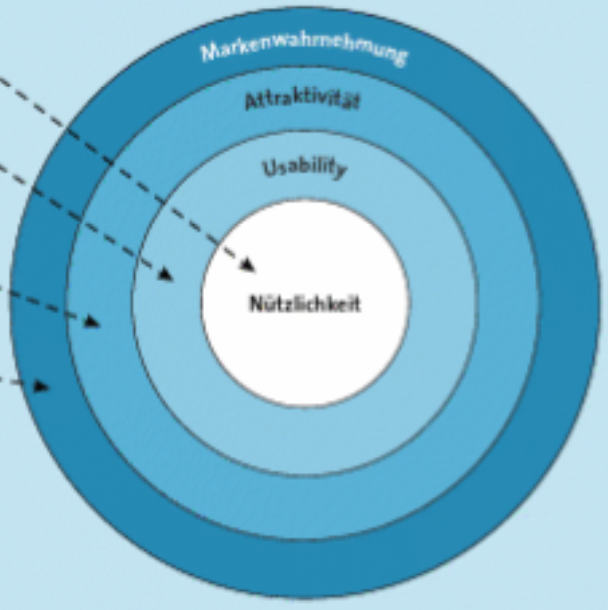
\includegraphics[height=8cm]{Bilder/User-Experience_Einflussfaktoren.png}
    \caption[Einflussfaktoren auf die User Experience]{Einflussfaktoren auf die User Experience. Darstellung nach \cite{theorie_beyer_user_experience_mit_sap_2020}}
    \label{fig:User-Experience_Einflussfaktoren}
\end{figure}

Die wichtigsten Faktoren sind Nützlichkeit und Usability, die sich unter dem Begriff Brauchbarkeit subsumieren lassen. Dieses Merkmal entscheidet hauptsächlich darüber, ob ein Anwender das Produkt wiederverwenden wird. Beide Komponenten müssen optimiert werden, da eine Anwendung, die zwar genau die gewünschte Funktionalität bietet, für einen User aber nicht bzw. nur sehr schwer bedienbar ist, nicht mehr genutzt wird. Andererseits ist ein Produkt, das sehr einfach zu bedienen ist, aber benötigte Funktionalitäten nicht bietet, ebenfalls nicht brauchbar. Wenn ein Anwender nachhaltig von dem Produkt überzeugt werden soll, muss dieses zudem attraktiv sein. Somit wird der Benutzer auf einer emotionalen Ebene an die Lösung gebunden und wird diese auch weiterhin nutzen. Eng zusammenhängend mit der Attraktivität eines Produkts ist dessen Markenwahrnehmung. Diese kann durch UX zwar nur indirekt beeinflusst werden, ist aber dennoch wichtig für eine langfristige Steigerung der Attraktivität. Letzteres kann zusammen mit einer positiven Markenwahrnehmung einen Anwender dazu bewegen, auch unter nach Nützlichkeits-Gesichtspunkten gleichwertigen Produktion, sich immer für ein bestimmtes Produkt zu entscheiden. \footcite[Vgl.][S. 51f]{theorie_beyer_user_experience_mit_sap_2020}

\subsubsection{Technology Acceptance Model}

Ein Modell, um die Akzeptanz von IT-Systemen durch Anwender zu erklären ist das Technology Acceptance Model (im Folgenden mit ''TAM'' abgekürzt).

\begin{figure}[H]
    \centering
    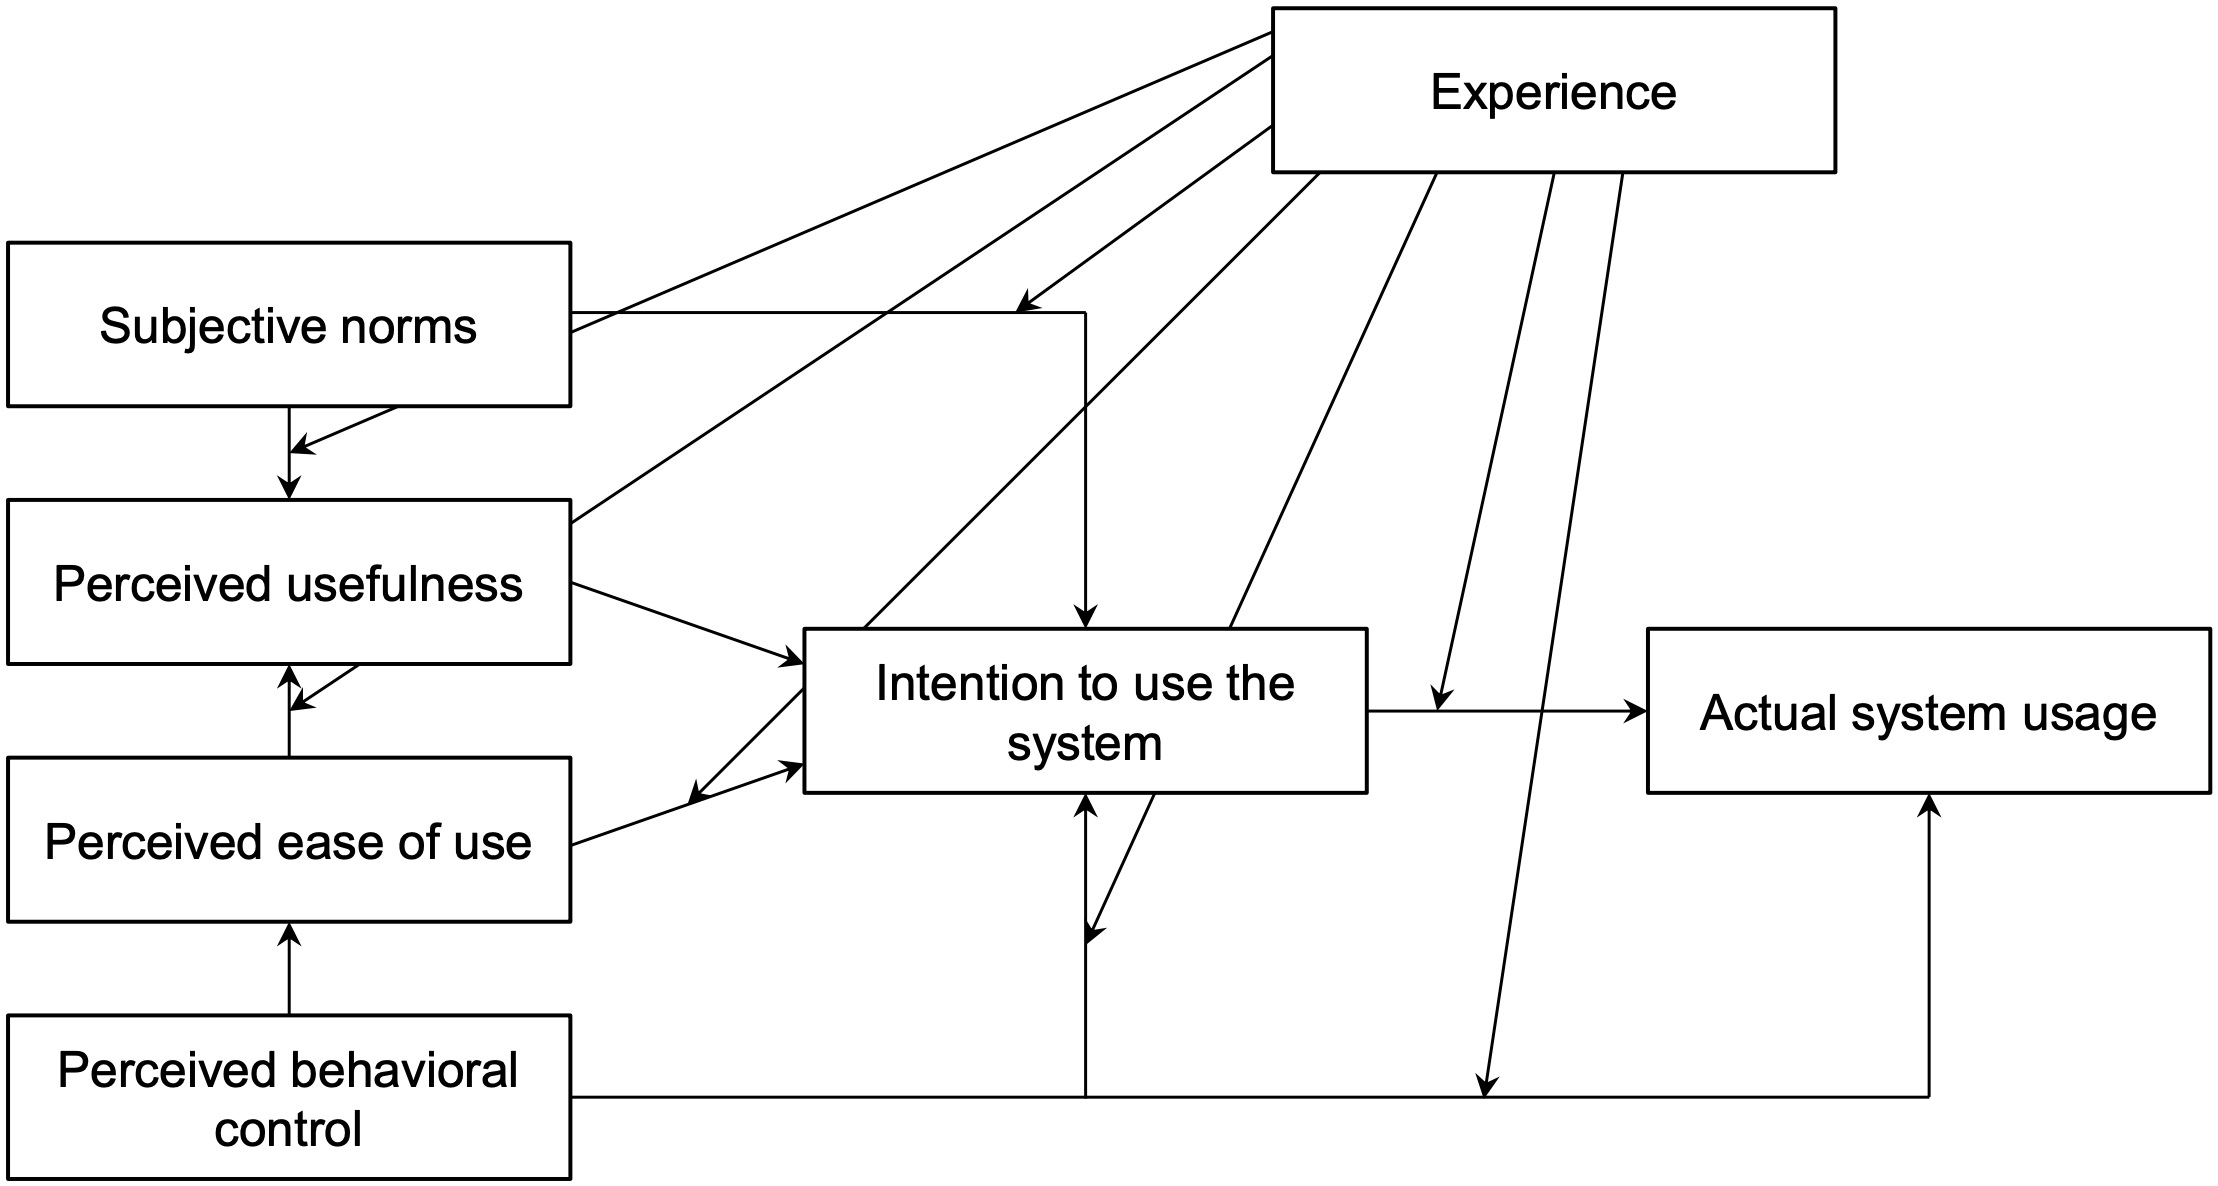
\includegraphics[height=8.02cm]{Bilder/User-Experience_ETAM.png}
    \caption[Extended Technology Acceptance Model]{Extended Technology Acceptance Model. Pfeile entsprechen Beziehungen zwischen Einflussfaktoren. Darstellung nach \cite[][]{theorie_kohnke_extended_tam_2023}}
    \label{fig:User-Experience_ETAM}
\end{figure}

Das TAM (s. Abbildung \ref{fig:User-Experience_ETAM}) wurde von \cite[][]{theorie_davis_tam_1989} entwickelt und bestimmt die 'wahrgenommene Nützlichkeit eines Systems' und die 'wahrgenommene Benutzerfreundlichkeit' als ausschlaggebende Faktoren für die Benutzung eines IT-Systems. Die wahrgenommene Nützlichkeit ist die subjektive Einschätzung eines Anwenders, dass die Nutzung des Systems seine berufliche Leistung verbessert, während die wahrgenommene Benutzerfreundlichkeit die subjektive Bewertung, inwiefern die Nutzung des Systems frei von Anstrengung ist, dargestellt. \footcite[Vgl.][S. 985]{theorie_davis_tam_1989}Diese beiden Aspekte beeinflussen die Absicht ein Produkt zu nutzen, was direkt die tatsächliche Nutzung beeinflusst. Im Bezug auf unternehmensübergreifend eingesetzte Standardsoftware wurde dieses ursprüngliche TAM um die Elemente 'subjektive Normen' und 'wahrgenommene Verhaltenskontrolle' zum Extended TAM (im Folgenden mit ''ETAM'' abgekürzt) erweitert. Subjektive Normen beschreiben die den Glauben einer Person, dass ihr wichtige Menschen eine Erwartungshaltung an sie haben, sich bestimmt zu verhalten. Somit beeinflussen diese Normen direkt die Absicht, ein System zu nutzen oder nicht. Die wahrgenommene Verhaltenskontrolle beschreibt die subjektive Einschätzung einer Person, dass sie in der Lage ist, ein bestimmtes Verhalten auszuführen. Diese Verhaltenskontrolle findet im beruflichen Kontext innerhalb interner und externer Verhaltensbeschränkungen statt. Verhaltensbeschränkungen können \zB durch Vorgaben des Arbeitgebers oder durch gesetzliche Regelungen entstehen. \footcite[Vgl.][S. 3f]{theorie_kohnke_extended_tam_2023} Ein Aspekt, der alle Faktoren des ETAM beeinflusst, ist die Erfahrung eines Nutzers. Beispielsweise beeinflusst die Benutzerfreundlichkeit eines Systems die Intention dieses zu nutzen bei einem unerfahrenen Anwender stärker als bei einem erfahrenen, da die Bedienung leichter erlernt werden kann.

\section{SAP Produktumfeld}

\subsubsection{SAP Ariba Direct Materials Sourcing for Automotive and Industrial Manufacturing in SAP S/4 HANA}

Die ''SAP Ariba Direct Materials Sourcing for Automotive and Industrial Manufacturing in SAP S/4 HANA''-Suite (im Folgenden mit ''DMS'' abgekürzt) ist ein Lösungs-Portfolio in der Cloud für die direkte Beschaffung in der Automobilindustrie und im produzierenden Gewerbe. Beschaffung meint in diesem Kontext strategische Handlungsfelder des Einkaufs. Solche sind \zB die Marktforschung, Lieferantenauswahl, Vertragsverhandlungen und Risikomanagement. \footcite[Vgl.][S. 541]{theorie_digitale_transformation_beschaffung_automobilindustrie_2019} Direkte Beschaffung bezeichnet den Einkauf von Gütern, die direkt in die Herstellung des Produkts eingehen, während indirekte Beschaffung den Einkauf von Gütern, die die Produktion unterstützen, beschreibt. \footcite[Vgl.][S. 541]{theorie_digitale_transformation_beschaffung_automobilindustrie_2019} Die DMS-Suite ist speziell für die Automobil- und Fertigungsindustrie konzipiert, da diese Branchen mit komplexen Produktionsprozessen und Bauteilen arbeiten und die Kooperation mit Lieferanten bei der Entwicklung neuer Produkte von gro\ss er Bedeutung ist. Mit S/4 HANA (im Folgenden mit ''S/4'' abgekürzt) als Basis kann gesamten Lebenszyklus der Bauteile, von der Produktentwicklung über die Beschaffung bis zum Qualitätsmanagement, abgedeckt werden. Das ermöglicht Kosteneinsparungen durch Effizienzsteigerung und ermöglicht ein transparentes Reporting des CO2-Fu\ss abdrucks. Zudem können alle Produkte durch das einheitliche Datenmodell einfach verknüpft werden. Durch die Vernetzung der Lösungen stehen alle Beschaffungsdaten in jedem System zur Verfügung und verbessern Entscheidungsfindung und Transparenz. \footcite[Vgl.][]{theorie_sap_webseite_dms_übersicht_2024}

\begin{figure}[H]
    \centering
    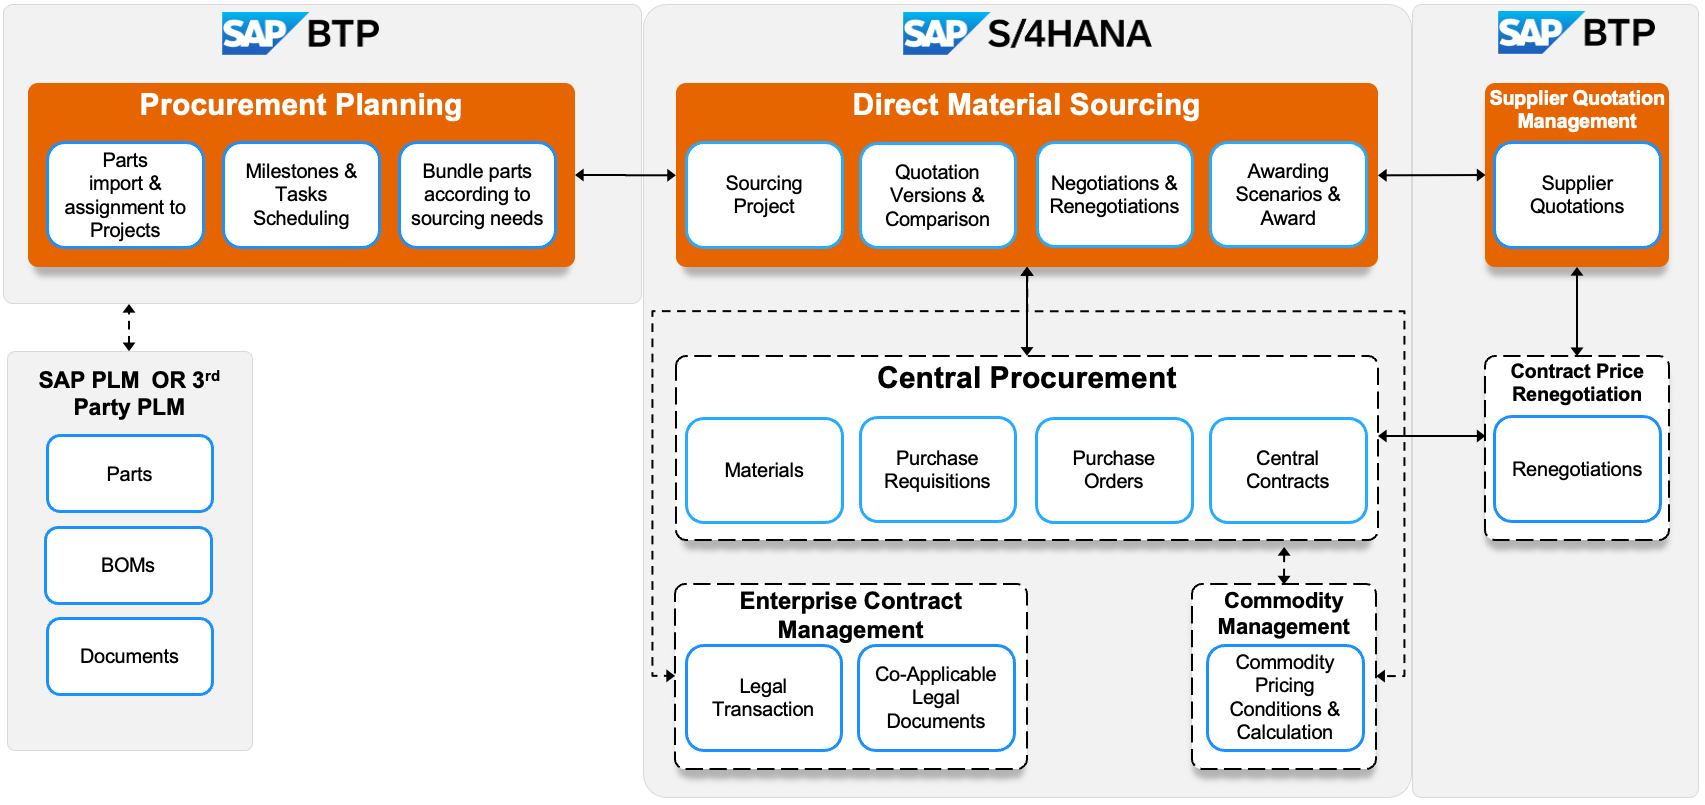
\includegraphics[height=7.09cm]{Bilder/Direct_Material_Sourcing_Overview3.png}
    \caption[SAP Ariba DMS Suite Produktübersicht]{SAP Ariba DMS Produktübersicht. Eigene Darstellung}
    \label{fig:Direct_Material_Sourcing_Overview3}
\end{figure}

Im Folgenden werden die einzelnen Bestandteile der Suite anhand Abbildung \ref{fig:Direct_Material_Sourcing_Overview3} beschrieben: Der Kern des Portfolios besteht aus den Produkten Procurement Planning, Direct Material Sourcing und Supplier Quotation Management. Optional kann vor Procurement Planning ein Product Lifecycle Management System von SAP oder einem Drittanbieter (im Folgenden ''PLM'' abgekürzt) integriert werden. In diesem System wird der gesamte Lebenszyklus des Produkts, von der Idee bis zum Support verwaltet. In diesem Kontext ist die Entwicklung von Bauteilen des Produkts und die Kollaboration mit Lieferanten relevant. \footcite[Vgl.][]{theorie_sap_plm_übersicht_2024} Aus dem PLM-System werden dann die benötigten Teile mit Spezifikationen in Procurement Planning übertragen. In Procurement Planning werden dann aus diesen Teile-Listen Beschaffungsprojekte erstellt. Innerhalb dieser Projekte wird der Bedarf und die dafür nötigen Finanzmittel über die Produktionsspanne des Produkts geplant. Durch das Setzen verschiedener Ziel-Daten werden Meilensteine rückwirkend geplant, sodass die Beschaffung anhand des Produktionsplans rechtzeitig erfolgt. \footcite[Vgl.][]{theorie_sap_procurement_planning_overview_2024} Nach der Planung, welche Mengen der verschiedenen Teile benötigt werden, werden diese in Beschaffungsprojekte gruppiert und in die Software Direct Material Sourcing übertragen. In diesem Schritt findet der eigentliche Einkauf statt. Die benötigten Bauteile werden ausgeschrieben und Lieferanten können in einem mehrstufigen Verfahren Angebote abgeben, bis dann nach mehreren Verhandlungsrunden ein Lieferant den Zuschlag erhält. \footcite[Vgl.][]{theorie_sap_webseite_dms_übersicht_2024} Die Verwaltung und Abgabe der Lieferantenangebote wird durch das Produkt Supplier Quotation Management unterstützt. Auf dieser Plattform können Lieferanten offene Ausschreibungen einsehen und Angebote abgeben. \footcite[Vgl.][]{theorie_sap_supplier_quotation_management_help_2024} Da viele Automobil- und Fertigungsunternehmen ihre Beschaffungsorganisation zentralisieren, kann Direct Material Sourcing mit dem Produkt Central Procurement verknüpft werden. Dadurch kann die Beschaffung über mehrere Standorte hinweg zentral gesteuert werden. Diese Lösung wird im nächsten Kapitel noch genauer beschrieben. Die Erstellung und Verwaltung legaler Verträge mit Lieferanten wird durch das Enterprise Contract Management unterstützt. Einkäufer können in Zusammenarbeit mit der Rechtsabteilung Verträge anhand von Vorlagen erstellen und zentralisiert verwalten. \footcite[Vgl.][]{theorie_sap_enterprise_contract_management_2024} Da viele Bauteile in der Industrie rohstoffintensiv sind, ist es möglich über das Produkt Commodity Management indexbasiert Preise für Rohstoffe mit den ausgeschriebenen Produkten zu verknüpfen, um Preisschwankungen abzufedern und daraus resultierende finanzielle Risiken zu minimieren. \footcite[Vgl.][]{theorie_sap_commodity_management_2024} Zuletzt ist noch die Lösung Contract Price Renegotiation zu nennen, durch die langfristige Verträge mit Lieferanten in festen Intervallen neu verhandelt werden können, um Preisänderungen, Effizienzsteigerungen und Skaleneffekten Rechnung zu tragen. Dadurch können für den Einkauf durch günstigere Kostenstrukturen Einsparungen erzielt werden. \footcite[Vgl.][]{theorie_sap_contract_price_renegotiation_2024}

\subsubsection{SAP Ariba Central Procurement}

SAP Ariba Central Procurement (im Folgenden ''CP'' abgekürzt) ist ein Produkt der DMS-Suite, welches die Zentralisierung der Beschaffung in einem Unternehmen ermöglicht. Gro\ss e Konzerne im Automobilsektor oder der Industrie haben meistens weltweit Tochtergesellschaften und Standorte mit jeweils eigenen IT-Systemen und Prozessen. Durch die Zentralisierung der Beschaffung können diese Prozesse vereinheitlicht und die IT-Systeme vernetzt werden. Durch die zentrale Steuerung der Beschaffungsorganisation werden Ineffizienzen vermieden, Kosten gespart und die Transparenz erhöht. Globale Richtlinien lassen sich einfacher durchsetzen und die Verhandlungsmacht gegenüber Lieferanten steigt durch gebündelte Bestell-Volumina. \footcite[Vgl.][]{theorie_sap_central_procurement_overview_2024}

\begin{figure}[H]
    \centering
    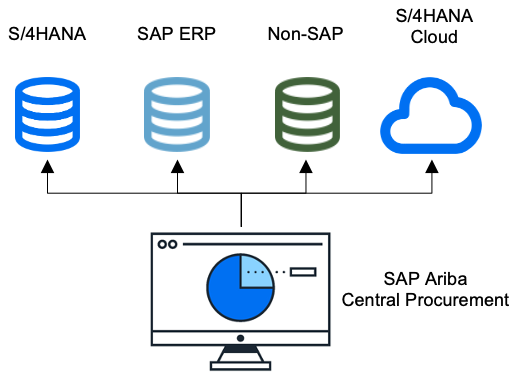
\includegraphics[height=6cm]{Bilder/Central_Procurement_System_Landscape.png}
    \caption[SAP Ariba Central Procurement Systemlandschaft]{SAP Ariba Central Procurement Systemlandschaft. Eigene Darstellung}
    \label{fig:Central_Procurement_System_Landscape}
\end{figure}

In einer bestehenden Systemlandschaft, wie in Abbildung \ref{fig:Central_Procurement_System_Landscape} dargestellt nimmt das CP-System die Rolle eines ''Hub''-Systems ein, das mit allen lokalen ERP-Systemen der einzelnen Standorte verbunden wird. Diese Systeme können SAP-Lösungen oder Systeme von Drittanbietern sein. Alle Beschaffungsdaten der lokalen Systeme sind in CP verfügbar und sind in beide Richtungen synchronisiert. CP besteht aus vier Sub-Lösungen: Central Requisitioning, Central Purchasing, Central Sourcing und Central Contracts. Central Requisitioning ermöglicht  das Sammeln aller Bestellanfragen der Standorte. Dadurch erhalten Einkäufer einen Überblick über den globalen Bedarf an bestimmten Teilen und können diesen gesammelt bei bestimmten Lieferanten beschaffen. Central Purchasing deckt diese Beschaffung ab, indem alle Bestellanforderungen in einer Bestellung gebündelt beschafft werden können. Mit Central Sourcing kann die Lieferantenauswahl zentral nach strategischen Gesichtspunkten gesteuert werden und so das Lieferkettenrisiko minimiert werden. So kann \zB für ein Bauteil immer bei einem bestimmten Lieferanten bestellt werden. Diese langfristigen Verträge werden durch Central Contracts abgebildet, die den Rahmen der Kooperation und Bedarfs-Mengen für mehrere Jahre festlegen. Diese dienen als Basis für konkrete Bestellungen aus den lokalen Systemen und alle Einkäufer der unterschiedlichen Tochtergesellschaften profitieren von den zentral verhandelten Konditionen. Des Weiteren bietet CP mit Central Analytics Analyse- und Reportingfunktionalitäten, um die Beschaffungsprozesse auf globaler Ebene zu überwachen und Optimierungspotenzial zu identifizieren, sowie einen Überblick über die globalen Beschaffungsausgaben zu erhalten. \footcite[Vgl.][]{theorie_sap_central_procurement_overview_2024}

\subsubsection{Central Contract}

Wie in den obigen Unterkapiteln beschrieben dienen Central Contracts als Rahmenverträge für längerfristige Kooperationen zwischen Lieferant und Kunde. Sie legen die Konditionen für die Beschaffung von bestimmten Bauteilen fest und sind die Basis für die Bestellungen aus den lokalen Systemen. Die Verträge enthalten Informationen, wie \zB Liefer- und Zahlungsbedingungen, welche Mengen in einem bestimmten Zeitraum für bestimmte Standorte geplant sind und wie sich die Preise aus bestimmten Zu- oder Abschlägen oder Index-Preisen zusammensetzen. Des weiteren sind die Zentralkontrakte auch mit den zugehörigen legalen Verträgen und lokalen Verträgen in den verbundenen Systemen verknüpft. \footcite[Vgl.][]{theorie_sap_central_contract_overview_2024}

\begin{figure}[H]
    \centering
    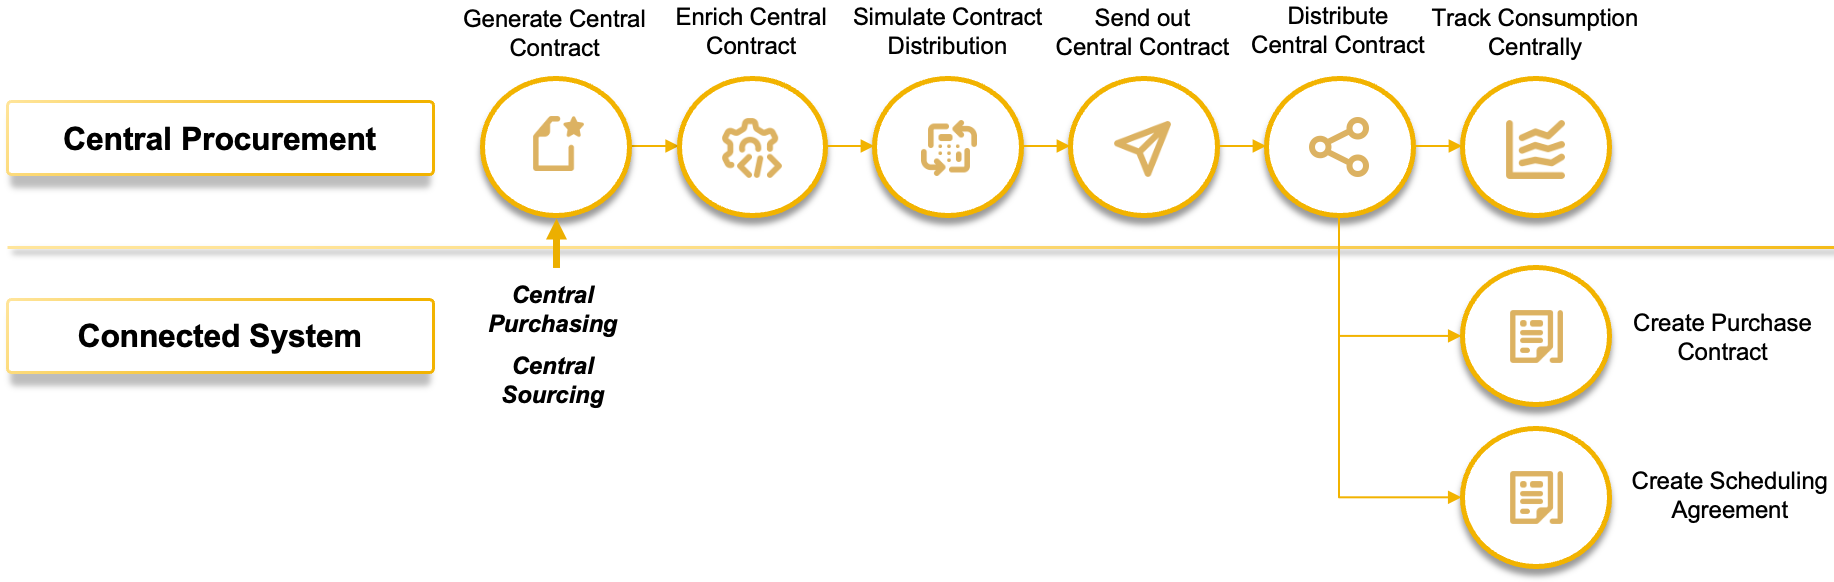
\includegraphics[height=4.76cm]{Bilder/Central_Contract_Process3.png}
    \caption[Central Contract Prozessübersicht]{Central Contract Prozessübersicht. Eigene Darstellung}
    \label{fig:Central_Contract_Process3}
\end{figure}

Der Prozess eines Central Contracts beginnt, wie Abbildung \ref{fig:Central_Contract_Process3} zeigt, mit der Erstellung eines neuen Vertrags aus einem Beschaffungsprojekt im Central Sourcing oder alternativ aus einer Bestellung im Central Purchasing. Zunächst muss der Kontrakt mit allen relevanten Daten angereichert werden. Dies geschieht meist über eine Schnittstelle zu den vorhergehenden Systemen, kann aber auch manuell durch einen Einkäufer erfolgen. Um sicherzustellen, dass die Replikation des Central Contracts in die lokalen Systeme fehlerfrei erfolgt, kann dies im nächsten Schritt simuliert werden. Nach erfolgreicher Simulation wird der Vertrag freigegeben und einerseits in die lokalen Back-End repliziert und andererseits den Lieferanten zur Verfügung gestellt. Dies löst die Erstellung von lokalen Verträgen in den jeweiligen Standorten als Pendant zum Central Contract aus, woraus dann die konkreten Bestellungen abgerufen werden. Die globalen Bestellvolumina können durch die Synchronisation im Zentralkontrakt überwacht werden.